% !TeX spellcheck = fr_FR

% TODO: Replace scan images with clean text where possible

\documentclass[a4paper, 10pt]{report}

\usepackage[french]{babel}
\usepackage[T1]{fontenc}

\usepackage{amsmath, amssymb, amsfonts}

\usepackage{hyperref}
\usepackage{geometry}

\usepackage{xcolor}
\usepackage{graphicx}

\usepackage{fancyhdr}
\usepackage{lastpage}

\usepackage{enumitem}

\geometry{
	a4paper,
	left=25mm,
	right=25mm,
	top=35mm,
	bottom=25mm,
	headsep=5mm,
	headheight=20mm,
}

\definecolor{solution}{HTML}{E5E4E2}
\providecommand{\abs}[1]{\lvert#1\rvert}
\providecommand{\norm}[1]{\lVert#1\rVert}
\DeclareMathOperator{\card}{card}

\begin{document}
	
	\renewcommand{\headrule}{%
		\vspace{-4pt}\hrulefill
		\raisebox{-6.8pt}{\ 
\includegraphics[height=5mm]{../../icon.png}}
		\hrulefill
	}	
	\pagestyle{fancy}
	\fancyhf{}
	
	\fancyhead[L]{\small \slshape Automne 2024}
	\fancyhead[C]{\Large \bfseries Analyse I - Série 09}
	\fancyhead[R]{\small Buff Mathias}
	\fancyfoot[L]{
		\small Source files available at:
		\href{https://github.com/MathiasBuff/bsc-math}
		{github.com/MathiasBuff/bsc-math}
	}
	\fancyfoot[R]{
		\small Page \thepage
		\hspace{1pt} /
		\pageref*{LastPage}
	}
	

	\noindent
	\textbf{Exercice 1.} Étudier les fonctions suivantes en trouvant
	leurs asymptotes et extremums locaux :
	\begin{enumerate}[label=(\roman*)]
		\item La fonction $x \mapsto 5x^2 - 10x + 15$.
		%
		\item La fonction $x \mapsto \frac{x^2 - 5x}{x^2 - 1}$.
	\end{enumerate}
	
	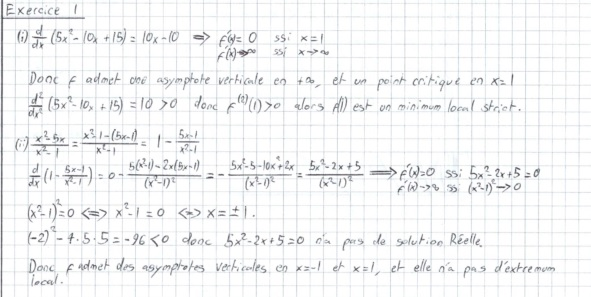
\includegraphics{ex01.jpg}
	
	\vspace{5mm}
	\noindent
	\textbf{Exercice 2.} En décomposant l'intervalle $[0, b]$ en $n$
	intervalles de longueurs égales, montrer à l'aide de l'Exercice
	4.1.(ii) que \[\int_{0}^{b}x^3 dx = \frac{b^4}{4}\]	
	
	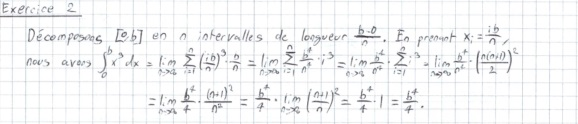
\includegraphics{ex02.jpg}
	
	\newpage
	
	\fancyhf{}
	\renewcommand{\headrule}
	{\rule{\textwidth}{0pt}}
	\fancyfoot[R]{
		\small Page \thepage
		\hspace{1pt} /
		\pageref*{LastPage}
	}
	
	\noindent
	\textbf{Exercice 3.} Montrer que
	\begin{equation}\label{eq1}
	\int_{a}^{b}x^p dx = \frac{b^{p+1} - a^{p+1}}{p+1}
	\end{equation}
	pour tout $b \geq a \geq 0$ et $p \in \mathbb{N}$, comme suit.
	\begin{enumerate}[label=(\roman*)]
		\item Montrer qu'il suffit de considérer $a > 0$.
		%
		\item Trouver la décomposition de $[a, b]$ en $n$ intervalles
		$I_1, \dotsc, I_n$, où $I_i$ a les bords $a_i$ et $a_{i+1}$,
		tels que le \textit{quotient} $a_{i+1}/a_i$ ne dépend pas de $i$.
		%
		\item En utilisant la décomposition de (ii) et l'expression pour
		la série géométrique, conclure \eqref{eq1} pour $b > a > 0$.
	\end{enumerate}
	
	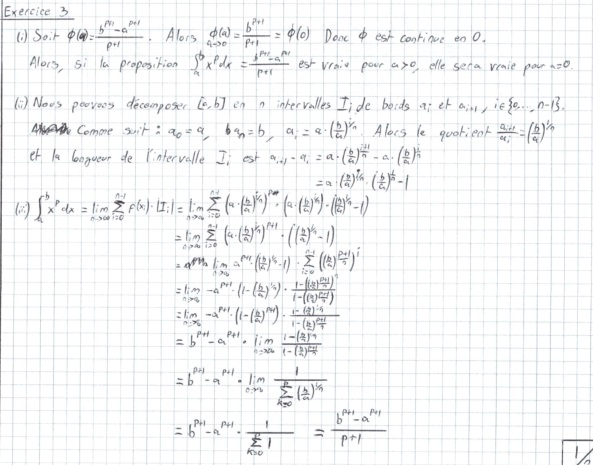
\includegraphics{ex03.jpg}
		
	\newpage
	
	\noindent
	\textbf{Exercice 4.} Déterminer si les fonctions $f$ suivantes
	définies sur $[0,1]$ sont intégrables. Justifier la réponse.
	\begin{enumerate}[label=(\roman*)]
		\item \[f(x) = \left\{\begin{aligned}
			&x &&\text{si } x \in \mathbb{Q}\\
			&0 &&\text{si } x \notin \mathbb{Q}
		\end{aligned}\right.\]
		%
		\item \[f(x) = \left\{\begin{aligned}
			&1 - \abs{2^{k+1}(x - 2^{-k}) - 1}&& \text{si }
			x \in [2^{-k}, 2^{-k+1}] \text{ pour } k \in \mathbb{N}^*\\
			&0&& \text{sinon}
		\end{aligned}\right.\]
		Commencer par dessiner le graphe de $f$.
	\end{enumerate}
	
	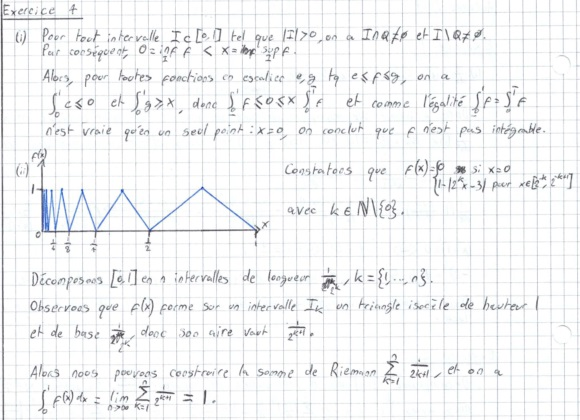
\includegraphics{ex04.jpg}
		
	\noindent
	\textbf{Exercice 5.} Montrer que la suite
	\[u_n = \sum_{i=1}^{n}\frac{n}{(n+i)^2}\]
	converge et exprimer sa limite comme une intégrale.
	
	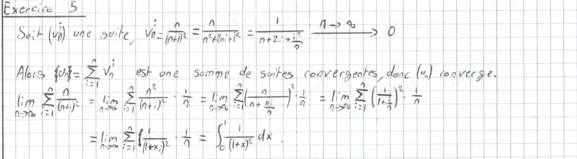
\includegraphics{ex05.jpg}
		
	\newpage
	
	\noindent
	\textbf{Exercice 6.} (Études de suites définies par récurrence)\\
	Soit $f$ une fonction $C^1$ et soit $\ell$ un point fixe de $f$,
	\textit{i.e.} $f(\ell) = \ell$. Définissons la suite $(u_n)$ par
	la relation de récurrence $u_{n+1} = f(u_n)$.
	\begin{enumerate}[label=(\roman*)]
		\item Supposons $\abs{f'(\ell) < 1}$.
		\begin{enumerate}[label=(\alph*)]
			\item Soit $\varepsilon > 0$ tel que
			$\abs{f'(\ell) < 1 - \varepsilon < 1}$. Montrer qu'il existe
			$\delta > 0$ tel que $\abs{f'(\ell) \leq 1 - \varepsilon}$
			pour tout $x \in [\ell - \delta, \ell + \delta]$. Nous fixons
			maintenant $\delta$ possédant cette propriété.
			%
			\item Montrer que si $u_N \in [\ell - \delta, \ell + \delta]$,
			alors
			$\abs{u_{n+1} - \ell} \leq (1 - \varepsilon)\abs{u_n - \ell}$
			pour tout $n \geq N$.
			%
			\item Montrer que
			$\abs{u_n - \ell} \leq (1 - \varepsilon)^n\abs{u_0 - \ell}$ si
			$u_0$ est assez proche de $\ell$. En déduire que pour $u_0$
			assez proche de $\ell, (u_n)$ tend vers $\ell$. On dit que le
			point fixe est \textit{attractif}.
		\end{enumerate}
		%
		\item Supposons $\abs{f'(\ell) > 1}$. Montrer en raisonnant
		par l'absurde que $(u_n)$ converge vers $\ell$ ssi\\
		$\exists N \in \mathbb{N}, \forall n \geq N, u_n = \ell$.
		Dans ce cas, le point fixe est dit \textit{répulsif}.
	\end{enumerate}
	
%	
%	
%	\colorbox{solution}
%	{
%		\begin{minipage}{0.9\textwidth}
%			s
%		\end{minipage}
%	}
%	
%	\colorbox{solution}
%	{
%		\begin{minipage}{0.9\textwidth}
%			\begin{enumerate}[label=(\alph*)]
%				\item a
%			\end{enumerate}
%		\end{minipage}
%	}
	
\end{document}
